\chapter{La sangre y el sistema circulatorio}\label{ch:b2:blood-circulation}

En 1628 William Harvey hizo una cuenta. El corazón, estimó, contiene unas
dos onzas de \omterm{def:b2:blood-circulation:blood}{sangre} y late setenta veces por minuto; aunque solo se
expulsara una fracción en cada latido, el corazón bombearía en una hora
varias veces el peso de todo el cuerpo. La \omterm{def:b2:blood-circulation:blood}{sangre} no podía fabricarse y
consumirse a ese ritmo, como había enseñado Galeno durante catorce
siglos; tenía que dar vueltas y más vueltas. Después lo demostró: si se
ata un cordón alrededor del brazo, las \omterm{def:b2:blood-circulation:vessels}{venas} se hinchan por debajo del
cordón, no por encima; si se empuja la \omterm{def:b2:blood-circulation:blood}{sangre} de una \omterm{def:b2:blood-circulation:vessels}{vena} hacia la mano,
más allá de una válvula, no pasa. La \omterm{def:b2:blood-circulation:blood}{sangre} sale bombeada por las
\omterm{def:b2:blood-circulation:vessels}{arterias}, vuelve por las \omterm{def:b2:blood-circulation:vessels}{venas}, y los cinco litros enteros pasan por el
corazón cada minuto. Este capítulo trata de ese sistema cerrado --- qué es
la \omterm{def:b2:blood-circulation:blood}{sangre}, cómo se distribuye, la física de su flujo por los vasos desde
la aorta hasta un \omterm{def:b2:blood-circulation:vessels}{capilar} y el intercambio, en los \omterm{def:b2:blood-circulation:vessels}{capilares}, que es la
razón de ser de todo ello.

\section{La sangre}

\begin{definition}[La composición de la sangre]\label{def:b2:blood-circulation:blood}
\index{sangre}\index{plasma}\index{hematocrito}\index{glóbulo rojo}\index{plaqueta}
La sangre es un tejido en suspensión: unos \qty{5}{L} en un adulto, el
\qty{7}{\%} de la masa corporal. Centrifugada, se separa en
\emph{plasma} (\qty{55}{\%}: agua, \qty{70}{g/L} de proteínas ---
albúmina, globulinas, fibrinógeno --- y las sales, azúcares, lípidos,
gases y hormonas que transporta) y células (\qty{45}{\%}, el
\emph{hematocrito}): \emph{glóbulos rojos} ($5\times 10^{12}$ por litro,
discos bicóncavos de \qty{7}{\micro m} sin núcleo, cada uno repleto de
\num{280} millones de moléculas de hemoglobina, que viven 120 días y se
fabrican en la médula ósea a razón de dos millones por segundo),
\emph{glóbulos blancos} ($7\times 10^{9}$ por litro: neutrófilos,
linfocitos, monocitos, eosinófilos, basófilos, el brazo móvil de la
inmunidad) y \emph{plaquetas} ($3\times 10^{11}$ por litro, fragmentos de
células de la médula que taponan las heridas e inician la coagulación).
Los glóbulos rojos transportan el oxígeno --- \qty{200}{mL} por litro de
sangre con saturación completa, setenta veces lo que disuelve el agua ---,
y el plasma transporta todo lo demás, incluido el \qty{20}{\%} del
$\mathrm{CO_2}$ que no está en las células, el calor de los músculos
hacia la piel y las hormonas del \cref{ch:b2:cell-signalling} hacia sus
dianas. La sangre es también una solución sometida a una \emph{\omterm{thm:b2:blood-circulation:oncotic}{presión
oncótica}}: sus proteínas, que no pueden salir de los \omterm{def:b2:blood-circulation:vessels}{capilares}, ejercen
unos \qty{25}{mmHg} de atracción osmótica, y esa atracción es lo que
mantiene el plasma dentro de los vasos.
\end{definition}

\begin{omfigure}
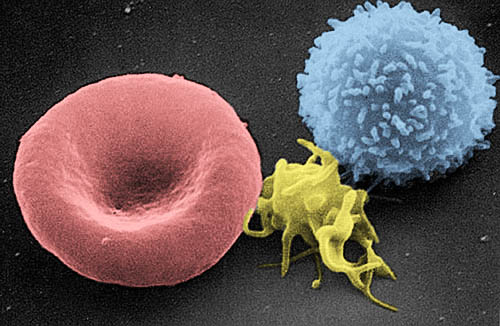
\includegraphics[width=0.5\linewidth]{images/book3/red-cells-nci.jpg}

{\small Un \omterm{def:b2:blood-circulation:blood}{glóbulo rojo}, una \omterm{def:b2:blood-circulation:blood}{plaqueta} y un glóbulo blanco (un linfocito)
al microscopio electrónico de barrido: los tres componentes celulares de
la \omterm{def:b2:blood-circulation:blood}{sangre}, a la misma escala.}
\end{omfigure}

\begin{proposition}[La hemostasia]\label{prop:b2:blood-circulation:clotting}
\index{hemostasia}\index{cascada de la coagulación}\index{fibrina}
Un vaso cortado se sella en tres etapas en pocos minutos. El vaso se
contrae; las \omterm{def:b2:blood-circulation:blood}{plaquetas} se adhieren al colágeno expuesto, liberan señales
que reclutan y activan más \omterm{def:b2:blood-circulation:blood}{plaquetas}, y forman un tapón; y una
\emph{cascada} de proteasas plasmáticas, cada una de las cuales activa a
la siguiente (una docena de factores de coagulación, la mayoría
fabricados en el hígado, varios dependientes de la vitamina K), convierte
el fibrinógeno en \emph{fibrina} insoluble, cuyos filamentos entrelazan el
tapón en un coágulo. Una cascada amplifica: una traza del
desencadenante (el factor tisular de la pared dañada) acaba en gramos de
fibrina. También debe contenerse: los anticoagulantes del \omterm{def:b2:blood-circulation:blood}{plasma}
(antitrombina, proteína C) y del endotelio intacto limitan el coágulo a la
herida, y un segundo sistema, la fibrinólisis, lo disuelve a medida que el
vaso cicatriza. La hemofilia es la falta de un factor; una trombosis es un
coágulo donde no debía haberlo, y la primera causa de muerte en los países
ricos es un coágulo en una \omterm{def:b2:blood-circulation:vessels}{arteria} coronaria o cerebral.
\end{proposition}

\section{Circuitos}

\begin{definition}[Abierta y cerrada, simple y doble]\label{def:b2:blood-circulation:circuits}
\index{circulación abierta}\index{circulación cerrada}\index{circulación doble}\index{circulación pulmonar}\index{circulación sistémica}
En una circulación \emph{abierta} (insectos, la mayoría de los moluscos)
un corazón bombea la \omterm{def:b2:blood-circulation:blood}{sangre} a una cavidad corporal donde baña
directamente los órganos y vuelve a baja presión; el flujo es lento y
está mal dirigido, y los insectos han separado el problema de los gases de
la \omterm{def:b2:blood-circulation:blood}{sangre} llevando el aire por tubos directamente hasta los tejidos. En
una circulación \emph{cerrada} (anélidos, cefalópodos, vertebrados) la
\omterm{def:b2:blood-circulation:blood}{sangre} permanece en los vasos y es impulsada a presión a través de los
\omterm{def:b2:blood-circulation:vessels}{capilares}, de modo que su distribución puede controlarse órgano por
órgano. Los peces tienen un circuito \emph{simple}: corazón
$\to$ branquias $\to$ cuerpo $\to$ corazón, de modo que la \omterm{def:b2:blood-circulation:blood}{sangre} llega a
los tejidos con la baja presión que queda tras los \omterm{def:b2:blood-circulation:vessels}{capilares} branquiales.
Los mamíferos y las aves tienen un circuito \emph{doble}: el corazón
derecho impulsa la circulación \emph{pulmonar} (pulmones, baja presión,
\qty{25}{mmHg} de sistólica) y el corazón izquierdo, cuando la \omterm{def:b2:blood-circulation:blood}{sangre}
regresa, impulsa la circulación \emph{sistémica} (cuerpo, alta presión,
\qty{120}{mmHg}); las dos bombas están en serie y mueven el mismo caudal,
unos \qty{5}{L} por minuto en reposo. Los anfibios y la mayoría de los
reptiles tienen un corazón con un solo ventrículo que mezcla en parte las
dos corrientes --- la etapa intermedia. El circuito doble es lo que hace
posible un metabolismo de sangre caliente: alta presión en todos los
órganos y un pulmón protegido de ella.
\end{definition}
\begin{proof}[Evidencia]
Harvey (1628) argumentó a partir de la cantidad --- el gasto calculado
más arriba --- y de la estructura: las válvulas de las \omterm{def:b2:blood-circulation:vessels}{venas}, que había
descrito Fabricius, solo permiten el flujo hacia el corazón, como mostró
presionando las \omterm{def:b2:blood-circulation:vessels}{venas} de un brazo ligado; las válvulas del corazón solo
permiten el flujo de las aurículas a los ventrículos y de estos a las
\omterm{def:b2:blood-circulation:vessels}{arterias}; y la \omterm{def:b2:blood-circulation:blood}{sangre} de las \omterm{def:b2:blood-circulation:vessels}{arterias} sale a borbotones, mientras que la
de las \omterm{def:b2:blood-circulation:vessels}{venas} rezuma. No podía ver los \omterm{def:b2:blood-circulation:vessels}{capilares} y dedujo su existencia;
Malpighi los vio en el pulmón de una rana en 1661, cuatro años después de
la muerte de Harvey.
\end{proof}

\begin{omfigure}
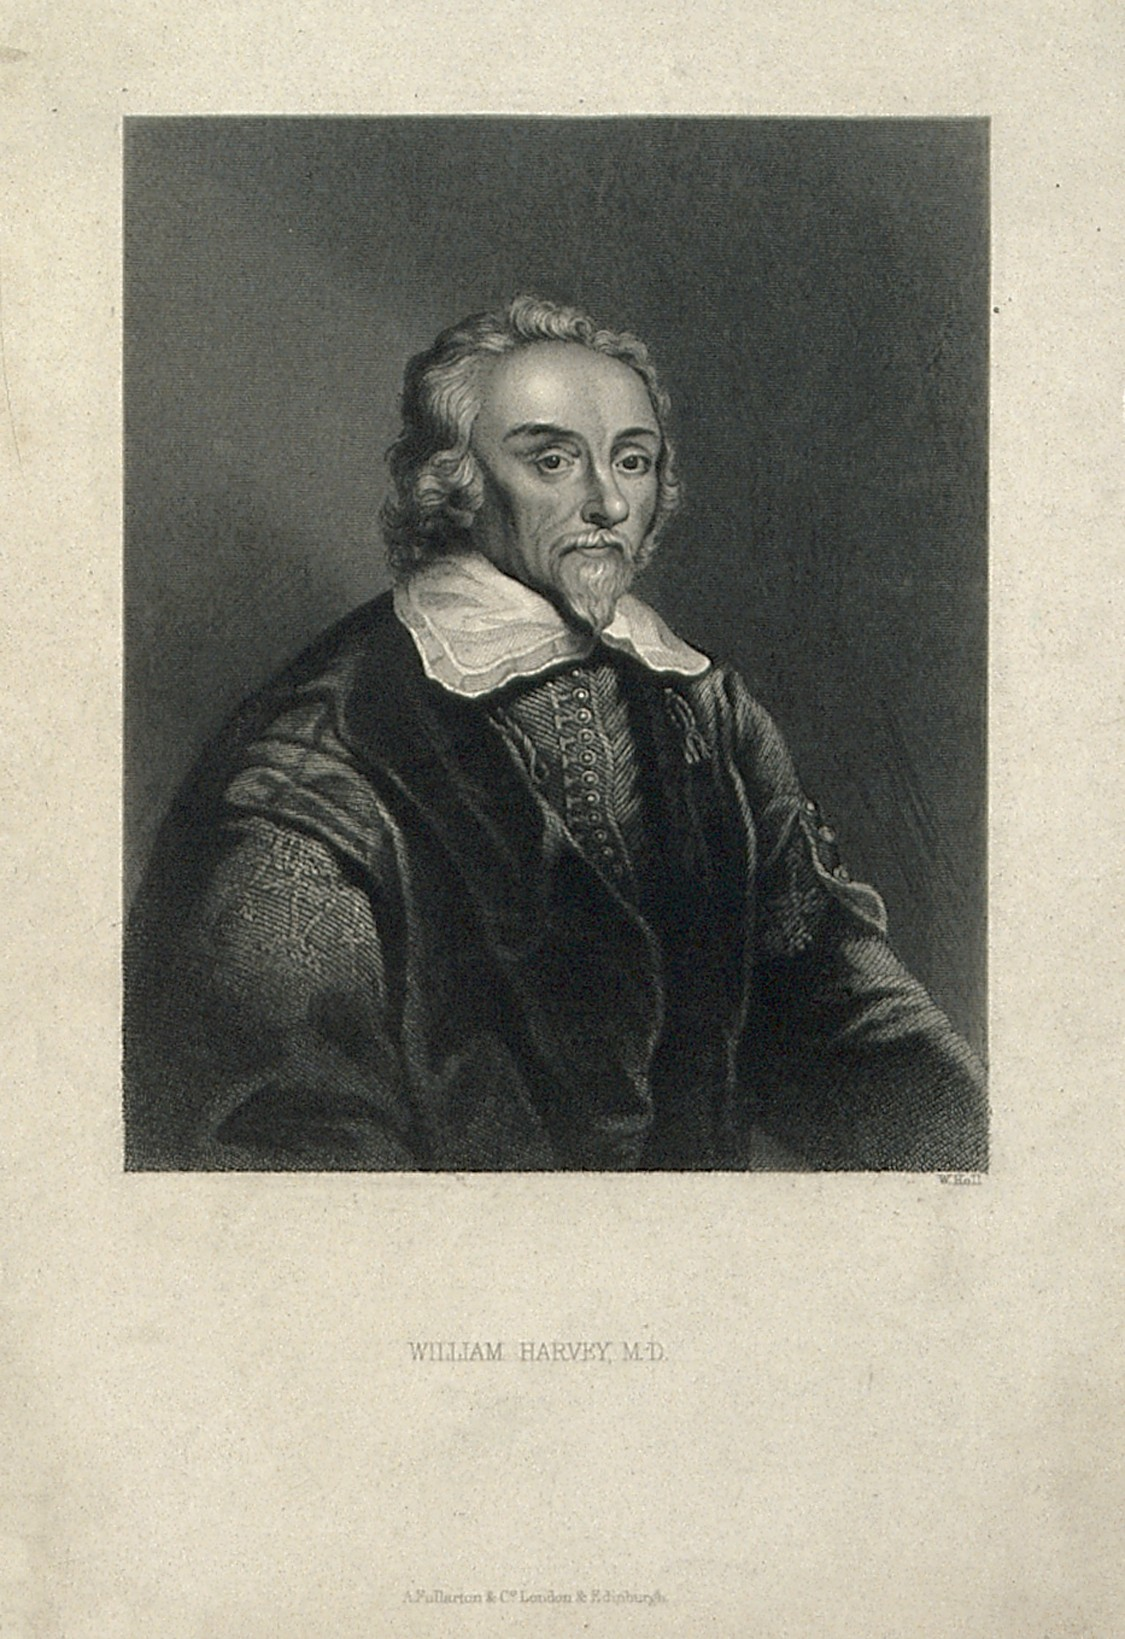
\includegraphics[width=0.3\linewidth]{images/book4/harvey.jpg}\hspace{0.05\linewidth}
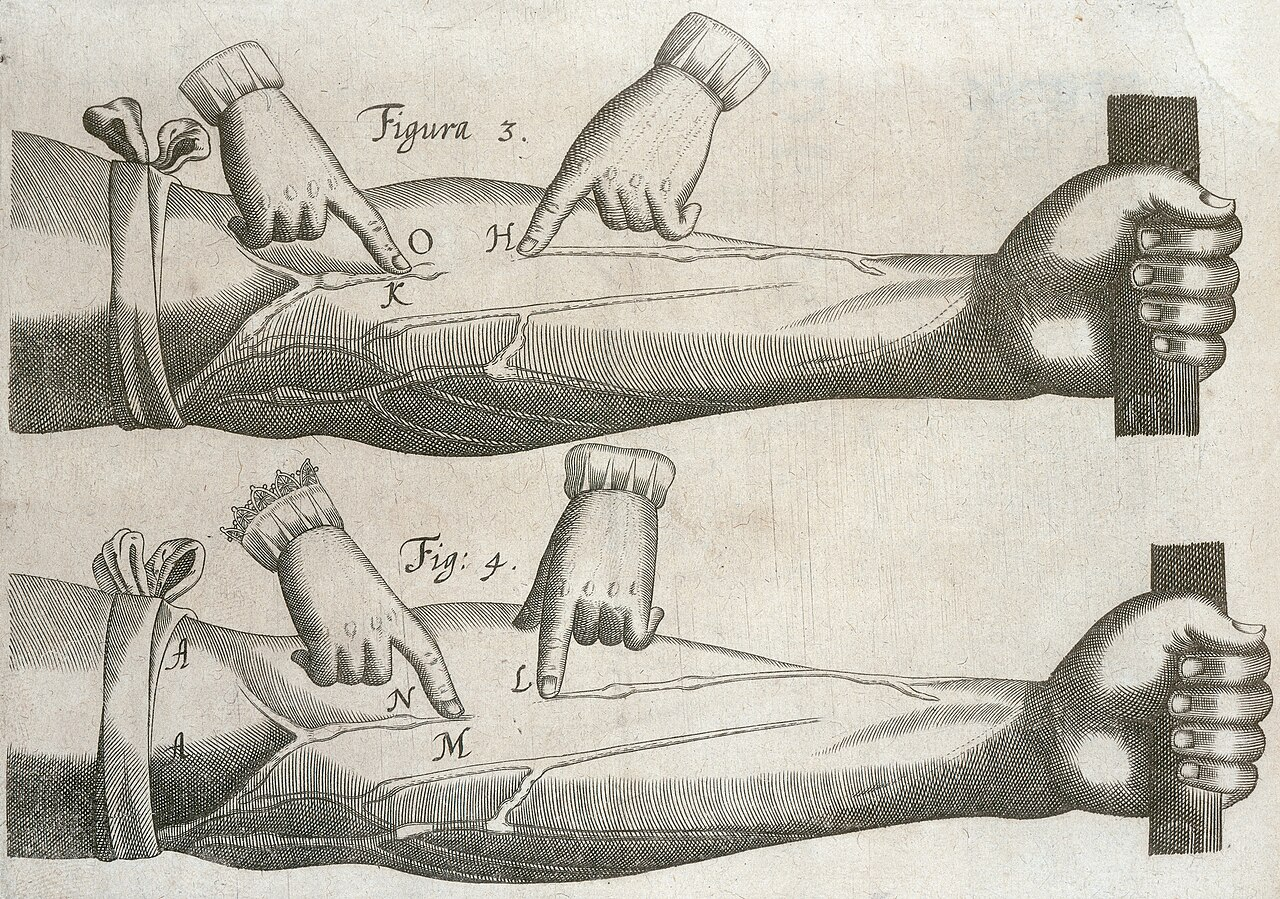
\includegraphics[width=0.42\linewidth]{images/book4/harvey-veins.jpg}

{\small William Harvey y la lámina de su libro de 1628: las \omterm{def:b2:blood-circulation:vessels}{venas} de un
antebrazo ligado se hinchan por debajo del cordón, y la \omterm{def:b2:blood-circulation:blood}{sangre} empujada
hacia la mano se detiene en las válvulas.}
\end{omfigure}

\begin{omfigure}
\begin{tikzpicture}[every node/.style={font=\scriptsize}, >=stealth]
  % lungs and body
  \node[draw, rounded corners, fill=omDef!12, minimum width=3.4cm, minimum height=0.9cm] (lung) at (0,3) {pulmones: capilares pulmonares};
  \node[draw, rounded corners, fill=omExo!25, minimum width=3.4cm, minimum height=0.9cm] (body) at (0,-3) {cuerpo: capilares sistémicos};
  % heart chambers
  \node[draw, fill=omDef!25, minimum width=1.3cm, minimum height=0.7cm] (ra) at (-1.6,0.6) {aurícula derecha};
  \node[draw, fill=omDef!35, minimum width=1.3cm, minimum height=0.9cm] (rv) at (-1.6,-0.5) {ventrículo derecho};
  \node[draw, fill=omThm!20, minimum width=1.3cm, minimum height=0.7cm] (la) at (1.6,0.6) {aurícula izquierda};
  \node[draw, fill=omThm!35, minimum width=1.3cm, minimum height=0.9cm] (lv) at (1.6,-0.5) {ventrículo izquierdo};
  \draw[->, thick] (ra) -- (rv); \draw[->, thick] (la) -- (lv);
  % pulmonary circuit
  \draw[->, very thick, omDef] (rv.west) -- ++(-1.4,0) |- (lung.west) node[pos=0.25, left, align=right] {arteria pulmonar\\\qty{25}{mmHg}};
  \draw[->, very thick, omThm] (lung.east) -| (la.east) node[pos=0.75, right, align=left] {venas pulmonares\\oxigenada};
  % systemic circuit
  \draw[->, very thick, omThm] (lv.east) -- ++(1.4,0) |- (body.east) node[pos=0.25, right, align=left] {aorta\\\qty{120}{mmHg}};
  \draw[->, very thick, omDef] (body.west) -| (ra.west);
  \node[omDef, anchor=east, align=right] at (-2.45,-1.6) {venas cavas\\\qty{5}{mmHg}};
  \node[anchor=north, align=center] at (0,-3.7) {el mismo caudal por ambos circuitos:\\\qty{5}{L/min} en reposo};
\end{tikzpicture}

{\small La \omterm{def:b2:blood-circulation:circuits}{circulación doble}. El corazón derecho envía la \omterm{def:b2:blood-circulation:blood}{sangre} a través
de los pulmones a baja presión; el corazón izquierdo la envía por el
cuerpo a alta presión; las dos bombas, en serie, mueven el mismo volumen
por minuto.}
\end{omfigure}

\section{Los vasos y la física del flujo}

\begin{definition}[El árbol vascular]\label{def:b2:blood-circulation:vessels}
\index{arteria}\index{arteriola}\index{capilar}\index{vena}
La \omterm{def:b2:blood-circulation:blood}{sangre} sale del corazón por las \emph{arterias}: tubos de pared gruesa
con capas elásticas que se estiran en cada latido y se retraen entre
latidos, suavizando los impulsos en un flujo más regular (la aorta mide
\qty{2.5}{cm} de diámetro). Se ramifican en \emph{arteriolas}, vasos de
una décima de milímetro o menos cuya pared es sobre todo músculo liso: al
contraerse o relajarse, una arteriola cambia su radio y, con él, de forma
muy marcada, su resistencia --- las arteriolas son los grifos de la
circulación y el lugar de la mayor parte de la caída de presión. Estas
desembocan en los \emph{capilares}: tubos de una sola célula endotelial
enrollada alrededor de una luz de \qtyrange{5}{10}{\micro m}, de alrededor
de \qty{1}{mm} de largo, unos cuarenta mil millones en total, con una
superficie total cercana a \qty{600}{m^2}, a través de cuyas paredes tiene
lugar todo el intercambio. Los capilares drenan en las vénulas y las
\emph{venas}: de pared delgada, distensibles, contienen dos tercios de la
\omterm{def:b2:blood-circulation:blood}{sangre} a baja presión, con válvulas que mantienen el flujo hacia el
corazón mientras los músculos las comprimen. Todo vaso está revestido de
una sola capa de \emph{endotelio}, que no es un revestimiento pasivo sino
una glándula --- libera óxido nítrico para relajar la arteriola y señales
que reclutan glóbulos blancos --- y un filtro.
\end{definition}

\begin{omfigure}
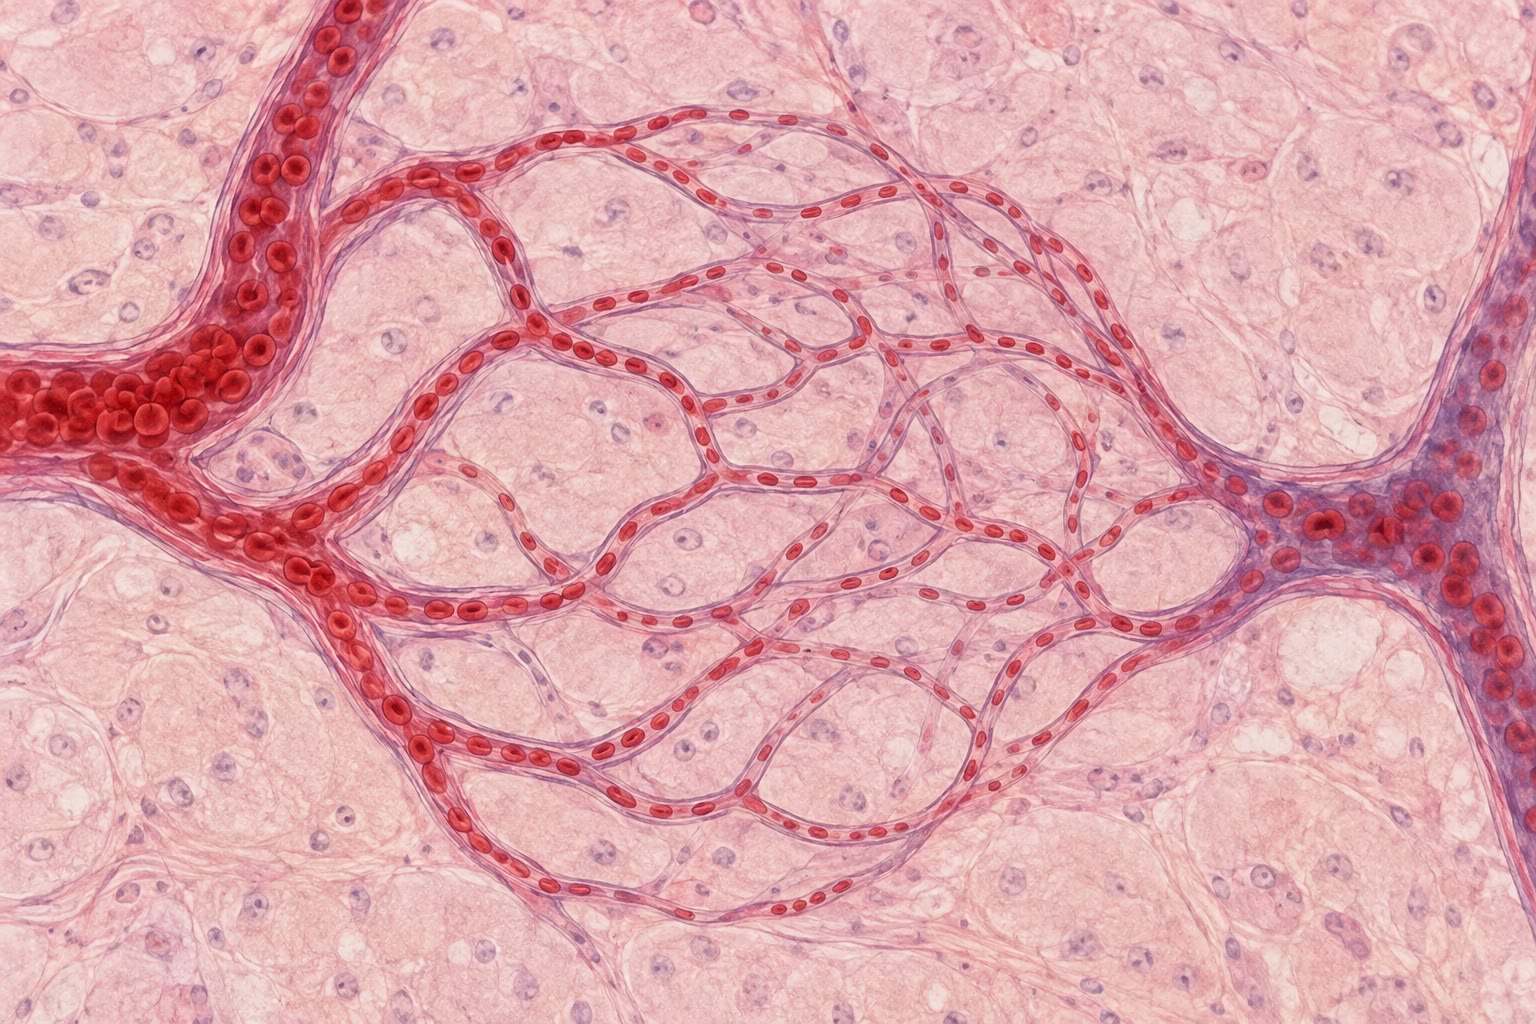
\includegraphics[width=0.55\linewidth]{images/book4/ai/b4-16-capillary-bed.jpg}

{\small Un lecho \omterm{def:b2:blood-circulation:vessels}{capilar}: una \omterm{def:b2:blood-circulation:vessels}{arteriola} que alimenta una red de \omterm{def:b2:blood-circulation:vessels}{capilares}
por los que los \omterm{def:b2:blood-circulation:blood}{glóbulos rojos} avanzan en fila india, y que vuelven a
reunirse en una vénula.}
\end{omfigure}

\begin{theorem}[La ley de Poiseuille y la resistencia vascular]\label{thm:b2:blood-circulation:poiseuille}
\index{ley de Poiseuille}\index{resistencia vascular}
El caudal estacionario $Q$ de un fluido de viscosidad $\eta$ a través de
un tubo de radio $r$ y longitud $L$ bajo una diferencia de presión
$\Delta P$ es
\[
Q = \frac{\pi r^{4}}{8\eta L}\,\Delta P, \qquad \text{de modo que}\qquad
R \equiv \frac{\Delta P}{Q} = \frac{8\eta L}{\pi r^{4}} .
\]
La resistencia disminuye con la \emph{cuarta potencia} del radio: una
\omterm{def:b2:blood-circulation:vessels}{arteriola} que reduce su radio un \qty{20}{\%} multiplica su resistencia
por $1/0.8^{4} = 2.4$, y una que lo reduce a la mitad, por 16. Por eso
unos pocos milímetros de músculo arteriolar pueden redirigir la \omterm{def:b2:blood-circulation:blood}{sangre} de
todo el cuerpo --- al intestino tras una comida, a los músculos durante el
ejercicio, a la piel con el calor ---, y por eso la presión cae de
\qty{95}{mmHg} en las pequeñas \omterm{def:b2:blood-circulation:vessels}{arterias} a \qty{35}{mmHg} a la entrada de
los \omterm{def:b2:blood-circulation:vessels}{capilares}, casi toda ella a través de las \omterm{def:b2:blood-circulation:vessels}{arteriolas}, mientras que la
caída a lo largo de la aorta es una fracción de milímetro de mercurio.
\end{theorem}
\begin{proof}
En un flujo laminar estacionario el fluido se desplaza en capas
concéntricas; la fuerza viscosa entre las capas equilibra la presión. Para
el cilindro de radio $s < r$, la fuerza de presión $\pi s^{2}\Delta P$
iguala el rozamiento viscoso sobre su superficie $2\pi s L\,\eta\,(-\mathrm{d}v/
\mathrm{d}s)$, de modo que $\mathrm{d}v/\mathrm{d}s = -s\Delta P/(2\eta L)$
y, con $v(r) = 0$, $v(s) = (\Delta P/4\eta L)(r^{2} - s^{2})$ --- un perfil
parabólico. Integrando la velocidad sobre la sección,
$Q = \int_{0}^{r} v\,2\pi s\,\mathrm{d}s = (\pi\Delta P/2\eta L)
\int_{0}^{r}(r^{2}s - s^{3})\,\mathrm{d}s = \pi r^{4}\Delta P/8\eta
L$. (La \omterm{def:b2:blood-circulation:blood}{sangre} no es exactamente un fluido simple y las \omterm{def:b2:blood-circulation:vessels}{arterias} no son
rígidas, pero la ley de la cuarta potencia se cumple lo bastante bien como
para hacer funcionar un cuerpo.)
\end{proof}

\begin{theorem}[Continuidad: dónde se frena la sangre]\label{thm:b2:blood-circulation:continuity}
\index{ecuación de continuidad}
Por cada nivel del árbol pasa el mismo volumen por segundo, de modo que la
velocidad media en un nivel es $v = Q/A$, donde $A$ es la sección
\emph{total} de todos los vasos de ese nivel. La aorta
(\qty{3}{cm^2}) transporta \qty{5}{L/min} a \qty{28}{cm/s}; los
\omterm{def:b2:blood-circulation:vessels}{capilares}, con una sección total cercana a \qty{3000}{cm^2}, lo
transportan a \qty{0.03}{cm/s}, de modo que un \omterm{def:b2:blood-circulation:blood}{glóbulo rojo} tarda unos tres
segundos en atravesar un \omterm{def:b2:blood-circulation:vessels}{capilar} --- tiempo suficiente para que su
oxígeno difunda hacia fuera (\cref{ch:b2:unicellular-diversity}: un
micrómetro en un milisegundo). Las \omterm{def:b2:blood-circulation:vessels}{venas}, de menor sección total que los
\omterm{def:b2:blood-circulation:vessels}{capilares}, vuelven a acelerar la \omterm{def:b2:blood-circulation:blood}{sangre} hasta \qty{10}{cm/s} en las \omterm{def:b2:blood-circulation:vessels}{venas}
cavas. El árbol está construido para que la \omterm{def:b2:blood-circulation:blood}{sangre} sea lenta justo donde
debe intercambiar y rápida en todas las demás partes.
\end{theorem}
\begin{proof}
Conservación del volumen: lo que entra en un nivel por segundo sale de él,
de modo que $Q = A\,v$ es igual en todos los niveles. $\qty{5}{L/min} =
\qty{83}{cm^3/s}$; $83/3 = \qty{28}{cm/s}$; $83/3000 =
\qty{0.028}{cm/s}$.
\end{proof}

\begin{omfigure}
\begin{tikzpicture}
\begin{axis}[
  width=0.9\linewidth, height=6.4cm,
  axis x line=bottom, axis y line=left,
  xmin=0, xmax=7, ymin=0, ymax=130,
  xtick={0.5,1.5,2.5,3.5,4.5,5.5,6.5},
  xticklabels={aorta, arterias, arteriolas, capilares, vénulas, venas, venas cavas},
  x tick label style={font=\scriptsize, rotate=30, anchor=north east},
  ylabel={presión (\unit{mmHg})}, ylabel style={font=\small, omThm},
  tick label style={font=\small}, ytick={0,40,80,120},
  legend style={font=\scriptsize, at={(0.97,0.95)}, anchor=north east, draw=none},
  clip=false,
]
\addplot[very thick, omThm] coordinates {(0,120) (0.5,118) (1,110) (1.5,100) (2,95) (2.5,60) (3,35) (3.5,25) (4,15) (4.5,12) (5,8) (5.5,5) (6,4) (6.5,3) (7,2)};
\addlegendentry{presión media}
\addplot[very thick, omThm, dashed] coordinates {(0,120) (0.5,120) (1,125) (1.5,120) (2,100)};
\addplot[very thick, omThm, dashed] coordinates {(0,80) (0.5,80) (1,80) (1.5,82) (2,88)};
\addlegendentry{sistólica y diastólica}
\end{axis}
\begin{axis}[
  width=0.9\linewidth, height=6.4cm,
  axis x line=none, axis y line=right,
  xmin=0, xmax=7, ymin=0, ymax=32,
  ylabel={velocidad (\unit{cm/s})}, ylabel style={font=\small, omDef},
  tick label style={font=\small}, ytick={0,10,20,30},
  legend style={font=\scriptsize, at={(0.97,0.72)}, anchor=north east, draw=none},
  clip=false,
]
\addplot[very thick, omDef] coordinates {(0,28) (0.5,26) (1,18) (1.5,10) (2,5) (2.5,1.5) (3,0.3) (3.5,0.03) (4,0.3) (4.5,1.5) (5,4) (5.5,7) (6,9) (6.5,10) (7,10)};
\addlegendentry{velocidad media}
\end{axis}
\end{tikzpicture}

{\small Presión (rojo) y velocidad media (azul) a lo largo de la
\omterm{def:b2:blood-circulation:circuits}{circulación sistémica}. El pulso se suaviza en las \omterm{def:b2:blood-circulation:vessels}{arterias}, la presión cae
sobre todo a través de las \omterm{def:b2:blood-circulation:vessels}{arteriolas}, y la \omterm{def:b2:blood-circulation:blood}{sangre} es más lenta en los
\omterm{def:b2:blood-circulation:vessels}{capilares}, donde la sección total es mil veces la de la aorta.}
\end{omfigure}

\begin{theorem}[La arteria elástica como depósito]\label{thm:b2:blood-circulation:windkessel}
\index{Windkessel}\index{distensibilidad!arterial}\index{presión del pulso}
El corazón expulsa a impulsos; los tejidos reciben un flujo casi
constante. Las grandes \omterm{def:b2:blood-circulation:vessels}{arterias} hacen el suavizado: se estiran durante la
eyección, almacenando parte del volumen sistólico, y se retraen durante la
diástole, impulsándolo hacia delante. Si las \omterm{def:b2:blood-circulation:vessels}{arterias} tienen una
\emph{distensibilidad} $C$ (volumen almacenado por unidad de presión) y las
\omterm{def:b2:blood-circulation:vessels}{arteriolas} una resistencia $R$, durante la diástole, con la válvula
aórtica cerrada, la presión decae como
\[
P(t) = P_{s}\,e^{-t/RC},
\]
de modo que la presión diastólica tras una diástole de duración $t_d$
es $P_s e^{-t_d/RC}$: con $R = \qty{1}{mmHg.s/mL}$, $C =
\qty{2}{mL/mmHg}$ y $t_d = \qty{0.8}{s}$, una sistólica de
\qty{120}{mmHg} cae a \qty{80}{mmHg}. Una aorta más rígida ($C$ menor, como
en la vejez) deja caer más la presión entre latidos y subir más durante la
eyección: la \emph{\omterm{thm:b2:blood-circulation:windkessel}{presión del pulso}} se ensancha, y el corazón trabaja
contra un pico más alto.
\end{theorem}
\begin{proof}
Durante la diástole no entra \omterm{def:b2:blood-circulation:blood}{sangre} en las \omterm{def:b2:blood-circulation:vessels}{arterias} y la \omterm{def:b2:blood-circulation:blood}{sangre} sale de
ellas a través de las \omterm{def:b2:blood-circulation:vessels}{arteriolas} a $Q = P/R$; el volumen arterial
disminuye a razón de $\mathrm{d}V/\mathrm{d}t = -P/R$ y, como $\mathrm{d}V = C\,
\mathrm{d}P$, $C\,\mathrm{d}P/\mathrm{d}t = -P/R$, cuya solución es la
exponencial de constante de tiempo $RC$. Con $RC = \qty{2}{s}$:
$120\,e^{-0.4} = \qty{80}{mmHg}$.
\end{proof}

\section{El intercambio en los capilares}

\begin{proposition}[Dos tipos de intercambio]\label{prop:b2:blood-circulation:exchange}
\index{intercambio capilar}\index{fuerzas de Starling}\index{edema}\index{linfa}
A través de la pared \omterm{def:b2:blood-circulation:vessels}{capilar}, los solutos se desplazan por
\emph{difusión} --- los gases y los lípidos a través de las células; el
agua y los solutos pequeños, por las hendiduras entre ellas ---, a lo largo
de la enorme superficie y la corta distancia que hacen abundante el flujo
(ley de Fick, como en la \omterm{def:b2:mammal-reproduction:placenta}{placenta} del
\cref{ch:b2:mammal-reproduction}), y el agua se desplaza por \emph{flujo
masivo}, impulsada por el equilibrio entre dos presiones. La presión
hidrostática del \omterm{def:b2:blood-circulation:vessels}{capilar}, $P_c$, empuja el líquido hacia fuera; la \omterm{thm:b2:blood-circulation:oncotic}{presión
oncótica} de las proteínas plasmáticas, $\pi_c$, lo atrae hacia dentro
(\emph{\omterm{prop:b2:blood-circulation:exchange}{fuerzas de Starling}}). En el extremo arterial, $P_c \approx
\qty{35}{mmHg}$ supera a $\pi_c \approx \qty{25}{mmHg}$ y el líquido se
filtra hacia fuera; en el extremo venoso, $P_c \approx \qty{15}{mmHg}$ y el
líquido se reabsorbe; en el conjunto del cuerpo se filtran unos
\qty{20}{L} al día y vuelven \qty{17}{L}, y el saldo de \qty{3}{L}, con las
proteínas que se han escapado, lo recogen los vasos \emph{linfáticos} y lo
devuelven a las \omterm{def:b2:blood-circulation:vessels}{venas} del cuello. El \emph{edema} --- la hinchazón por
líquido en los tejidos --- aparece siempre que el equilibrio se rompe:
presión venosa alta (insuficiencia cardíaca), proteínas plasmáticas bajas
(desnutrición, enfermedad hepática o renal), \omterm{def:b2:blood-circulation:vessels}{capilares} permeables
(inflamación) o linfáticos obstruidos.
\end{proposition}
\begin{omfigure}
\begin{tikzpicture}[every node/.style={font=\scriptsize}, >=stealth]
  % capillary
  \draw[thick, fill=omThm!10] (0,0) rectangle (9,1.2);
  \node[left] at (-0.1,0.6) {arteriola};
  \node[right] at (9.1,0.6) {vénula};
  \draw[->, very thick, omThm] (0.3,0.6) -- (8.7,0.6);
  % pressures
  \node[above, align=center] at (1.5,1.3) {extremo arterial\\$P_c = 35$, $\pi_c = 25$};
  \node[above, align=center] at (7.5,1.3) {extremo venoso\\$P_c = 15$, $\pi_c = 25$};
  \foreach \x in {0.8,1.5,2.2} \draw[->, thick, omDef] (\x,0) -- (\x,-0.7);
  \node[below, align=center, omDef] at (1.5,-0.75) {neta $+10$ mmHg:\\filtración};
  \foreach \x in {6.8,7.5,8.2} \draw[->, thick, omDef] (\x,-0.7) -- (\x,0);
  \node[below, align=center, omDef] at (7.5,-0.75) {neta $-10$ mmHg:\\reabsorción};
  \draw[->, thick, omExo!70!black] (4.5,-0.4) -- (4.5,-1.6) node[below, align=center] {exceso hacia la linfa:\\\qty{3}{L} al día};
  \node[align=center] at (4.5,-0.15) {líquido intersticial};
\end{tikzpicture}

{\small Las \omterm{prop:b2:blood-circulation:exchange}{fuerzas de Starling} a lo largo de un \omterm{def:b2:blood-circulation:vessels}{capilar}. La presión
hidrostática empuja el líquido hacia fuera y la \omterm{thm:b2:blood-circulation:oncotic}{presión oncótica} de las
proteínas plasmáticas lo atrae de vuelta; la filtración en el extremo
arterial supera a la reabsorción en el extremo venoso, y la linfa devuelve
la diferencia.}
\end{omfigure}

\begin{theorem}[La presión oncótica]\label{thm:b2:blood-circulation:oncotic}
\index{presión oncótica}\index{albúmina}
Una solución de $c$ moles por litro de un soluto que no puede atravesar una
membrana ejerce a través de ella una presión osmótica $\pi = cRT$ (van 't
Hoff). La albúmina del \omterm{def:b2:blood-circulation:blood}{plasma}, \qty{40}{g/L} de una proteína de masa molar
\qty{66}{kg/mol}, supone $c = \qty{0.6}{mmol/L}$ y da $\pi =
0.6\times 8.314\times 310 = \qty{1.55}{kPa} \approx \qty{12}{mmHg}$;
las demás proteínas y los iones adicionales que retiene la carga negativa
de la albúmina elevan el total a unos \qty{25}{mmHg}. El cloruro de sodio
del \omterm{def:b2:blood-circulation:blood}{plasma}, a \qty{150}{mmol/L}, ejercería \qty{5800}{mmHg} --- pero
atraviesa libremente la pared \omterm{def:b2:blood-circulation:vessels}{capilar} y no ejerce ninguna a través de
ella. Lo que importa para el \omterm{def:b2:blood-circulation:vessels}{capilar} son las proteínas: si la albúmina se
reduce a la mitad, como en la enfermedad renal que la pierde por la orina,
la atracción reabsorbente se reduce a la mitad, el líquido se acumula en
los tejidos y el paciente se hincha.
\end{theorem}
\begin{proof}
$\qty{40}{g/L}/\qty{66000}{g/mol} = \qty{6.1e-4}{mol/L} =
\qty{0.61}{mol/m^3}$; $\pi = cRT = 0.61\times 8.314\times 310 =
\qty{1570}{Pa}$; $\qty{1}{mmHg} = \qty{133}{Pa}$, luego \qty{11.8}{mmHg}.
La propia ley de van 't Hoff es el límite de las soluciones diluidas
deducido en el volumen del primer año.
\end{proof}

\begin{example}[La circulación como sistema de transporte]\label{ex:b2:blood-circulation:transport}
Cinco litros por minuto a través de \qty{600}{m^2} de pared \omterm{def:b2:blood-circulation:vessels}{capilar} son un
servicio de reparto sin igual. Lleva a cada célula oxígeno a unos pocos
diámetros celulares de distancia (ninguna célula del cuerpo está a más de
\qty{20}{\micro m} de un \omterm{def:b2:blood-circulation:vessels}{capilar}), retira su $\mathrm{CO_2}$, su lactato y
su urea, lleva la glucosa del hígado al encéfalo y los ácidos grasos de las
reservas de grasa a los músculos, distribuye en un minuto las hormonas del
\cref{ch:b2:cell-signalling} desde una glándula hasta cada receptor del
cuerpo, desplaza el calor del núcleo corporal a la piel y de vuelta, y
lleva los glóbulos blancos a una herida en pocas horas. Es también su
vulnerabilidad: un coágulo, una hemorragia o una bomba que falla lo
detienen todo a la vez, y el encéfalo, que no almacena combustible, falla
en segundos. El resto de esta parte del libro trata de la bomba
(\cref{ch:b2:heart}) y de cómo se regula la presión para que el servicio
continúe al ponerse de pie, al correr y al sangrar
(\cref{ch:b2:blood-pressure}).
\end{example}

\section{Ejercicios}

\begin{exercise}[$\star$]\label{exo:b2:blood-circulation:1}
Dese la composición de la \omterm{def:b2:blood-circulation:blood}{sangre} en volumen y el número, el tamaño y la
función de cada componente celular.
\end{exercise}

\begin{exercise}[$\star$]\label{exo:b2:blood-circulation:2}
Dibújense el circuito de un pez y el de un mamífero, márquense las
presiones y dígase qué aporta el circuito doble.
\end{exercise}

\begin{exercise}[$\star$]\label{exo:b2:blood-circulation:3}
Para cada tipo de vaso --- \omterm{def:b2:blood-circulation:vessels}{arteria}, \omterm{def:b2:blood-circulation:vessels}{arteriola}, \omterm{def:b2:blood-circulation:vessels}{capilar}, \omterm{def:b2:blood-circulation:vessels}{vena} ---, dense la
estructura de la pared y la función a la que sirve.
\end{exercise}

\begin{exercise}[$\star$]\label{exo:b2:blood-circulation:4}
Reconstrúyase el argumento de Harvey a partir de la cantidad, con cifras
modernas: \qty{70}{mL} por latido, \num{72} latidos por minuto, \qty{5}{L}
de \omterm{def:b2:blood-circulation:blood}{sangre}.
\end{exercise}

\begin{exercise}[$\star\star$]\label{exo:b2:blood-circulation:5}
Calcúlese mediante la \omterm{thm:b2:blood-circulation:poiseuille}{ley de Poiseuille} la caída de presión a lo largo de
la aorta (radio de \qty{1.25}{cm}, longitud de \qty{40}{cm},
$\eta = \qty{3e-3}{Pa.s}$) cuando transporta
\qty{5}{L/min}, en pascales y en mmHg. Coméntese.
\end{exercise}

\begin{exercise}[$\star\star$]\label{exo:b2:blood-circulation:6}
Una \omterm{def:b2:blood-circulation:vessels}{arteriola} de \qty{15}{\micro m} de radio se contrae hasta
\qty{12}{\micro m} y después se dilata hasta \qty{20}{\micro m}. ¿En qué
factor cambian en cada caso su resistencia y, a presión constante, su
caudal?
\end{exercise}

\begin{exercise}[$\star\star$]\label{exo:b2:blood-circulation:7}
La aorta tiene una sección de \qty{3}{cm^2} y los \omterm{def:b2:blood-circulation:vessels}{capilares}, una sección
total de \qty{3000}{cm^2}; el caudal es de \qty{5}{L/min}. Calcúlense la
velocidad media en cada uno y el tiempo que pasa un \omterm{def:b2:blood-circulation:blood}{glóbulo rojo} en un
\omterm{def:b2:blood-circulation:vessels}{capilar} de \qty{1}{mm}. Durante el ejercicio, el gasto sube a
\qty{25}{L/min} y se abren los \omterm{def:b2:blood-circulation:vessels}{capilares} musculares: ¿qué le ocurre al
tiempo de tránsito?
\end{exercise}

\begin{exercise}[$\star\star$]\label{exo:b2:blood-circulation:8}
Con $P_c = 35$ y \qty{15}{mmHg} en los dos extremos, $\pi_c =
\qty{25}{mmHg}$ y presiones intersticiales despreciables, calcúlese la
presión neta de filtración en cada extremo. ¿Qué ocurre si la presión
venosa sube de modo que $P_c$ en el extremo venoso es de \qty{28}{mmHg}?
\end{exercise}

\begin{exercise}[$\star\star$]\label{exo:b2:blood-circulation:9}
Calcúlese la \omterm{thm:b2:blood-circulation:oncotic}{presión oncótica} de \qty{40}{g/L} de albúmina
(\qty{66}{kg/mol}) a \qty{37}{\celsius}, y la de \qty{20}{g/L}. ¿Por qué
el sodio del \omterm{def:b2:blood-circulation:blood}{plasma}, a \qty{150}{mmol/L}, no contribuye en nada al
equilibrio de Starling?
\end{exercise}

\begin{exercise}[$\star\star\star$]\label{exo:b2:blood-circulation:10}
Con $R = \qty{1}{mmHg.s/mL}$ y $C = \qty{2}{mL/mmHg}$, calcúlese la
presión diastólica al cabo de \qty{0.8}{s} a partir de una sistólica de
\qty{120}{mmHg}. Vuélvase a calcular para una aorta la mitad de distensible.
Explíquese por qué la \omterm{thm:b2:blood-circulation:windkessel}{presión del pulso} de las personas mayores es amplia,
y lo que le cuesta al corazón.
\end{exercise}

\begin{exercise}[$\star\star\star$]\label{exo:b2:blood-circulation:11}
La resistencia sistémica es $R = (P_{\text{art}} - P_{\text{ven}})/Q$.
Calcúlese en reposo ($95 - 5$ mmHg, \qty{5}{L/min}) y durante el ejercicio
($110 - 5$, \qty{25}{L/min}). ¿En qué factor ha debido cambiar el radio
arteriolar medio, si las \omterm{def:b2:blood-circulation:vessels}{arteriolas} soportan toda la resistencia?
\end{exercise}

\begin{exercise}[$\star\star\star$]\label{exo:b2:blood-circulation:12}
``La circulación está construida para que la \omterm{def:b2:blood-circulation:blood}{sangre} sea lenta donde debe
intercambiar y rápida en todas las demás partes.'' Discútase con la
\omterm{thm:b2:blood-circulation:continuity}{ecuación de continuidad}, la \omterm{thm:b2:blood-circulation:poiseuille}{ley de Poiseuille} y la geometría del árbol, y
dígase por qué una \omterm{def:b2:blood-circulation:circuits}{circulación abierta} no puede hacer lo mismo.
\end{exercise}

\section{Problema: la circulación en cifras}

\begin{problem}[{Problema de fin de semana --- se rehace la cuenta de
Harvey, se calculan las presiones y las velocidades del árbol vascular con
Poiseuille y la continuidad, se hace el balance de la filtración diaria de
los capilares y se modeliza el suavizado de la aorta, hasta llegar al gasto
cardíaco, la caída de presión arteriolar, el filtrado del día y la presión
diastólica}]
\label{pb:b2:blood-circulation:1}
Datos: volumen sistólico de \qty{70}{mL}, frecuencia cardíaca de
\qty{72}{min^{-1}}, volumen sanguíneo de \qty{5}{L},
$\eta = \qty{3e-3}{Pa.s}$, $\qty{1}{mmHg} =
\qty{133}{Pa}$. Aorta: radio de \qty{1.25}{cm}, longitud de \qty{40}{cm}.
\omterm{def:b2:blood-circulation:vessels}{Arteriolas}: $3\times 10^{6}$ en paralelo, cada una de \qty{15}{\micro m}
de radio y \qty{1}{mm} de longitud. \omterm{def:b2:blood-circulation:vessels}{Capilares}: $4\times
10^{10}$, de \qty{3}{\micro m} de radio y \qty{1}{mm} de longitud, con la
cuarta parte abiertos en reposo. Starling: $P_c$ de 35 a \qty{15}{mmHg}
a lo largo de un \omterm{def:b2:blood-circulation:vessels}{capilar}, $\pi_c = \qty{25}{mmHg}$. Windkessel: $C =
\qty{2}{mL/mmHg}$, diástole de \qty{0.8}{s}.

\medskip
\noindent\textbf{Parte I --- La cuenta de Harvey.}
\begin{enumerate}
  \item Calcúlese el gasto cardíaco en litros por minuto y por día.
  \item ¿Cuántas veces circula el volumen sanguíneo en un día?
  \item La estimación de Harvey era de 2~onzas (\qty{57}{g}) por latido,
        de las que suponía que se expulsaba al menos la cuarta parte, a 72
        latidos por minuto. ¿Qué masa de \omterm{def:b2:blood-circulation:blood}{sangre} daba eso por hora, y cómo se
        comparaba con el peso de un hombre?
  \item ¿Por qué era esto un argumento a favor de la circulación y no de
        una producción y un consumo continuos?
  \item Descríbanse el experimento de la ligadura y lo que mostraban las
        válvulas.
  \item ¿Qué no podía ver Harvey, y quién lo vio?
\end{enumerate}

\medskip
\noindent\textbf{Parte II --- El árbol.}
\begin{enumerate}[resume]
  \item Calcúlese la velocidad media en la aorta.
  \item Calcúlese mediante la \omterm{thm:b2:blood-circulation:poiseuille}{ley de Poiseuille} la caída de presión a lo
        largo de la aorta, en mmHg.
  \item Calcúlense la resistencia de una \omterm{def:b2:blood-circulation:vessels}{arteriola} y la de las $3\times
        10^{6}$ en paralelo.
  \item Calcúlese la caída de presión a través de las \omterm{def:b2:blood-circulation:vessels}{arteriolas} con el
        gasto en reposo, en mmHg.
  \item Calcúlense la sección total de los \omterm{def:b2:blood-circulation:vessels}{capilares} abiertos y la
        velocidad media en ellos; después, el tiempo de tránsito por uno
        de ellos.
  \item Las \omterm{def:b2:blood-circulation:vessels}{arteriolas} se contraen de modo que su radio disminuye un
        \qty{10}{\%}. Vuélvase a calcular la caída. ¿Qué debe hacer el
        corazón para mantener el mismo gasto?
\end{enumerate}

\medskip
\noindent\textbf{Parte III --- Los \omterm{def:b2:blood-circulation:vessels}{capilares}.}
\begin{enumerate}[resume]
  \item Calcúlese la presión neta de filtración en el extremo arterial,
        en el extremo venoso y en el punto medio (tómese una caída lineal
        de $P_c$).
  \item Divídase el \omterm{def:b2:blood-circulation:vessels}{capilar} en la mitad que filtra y la mitad que
        reabsorbe, y estímense el líquido filtrado y el reabsorbido al día
        en todo el cuerpo, tomando como presiones netas promediadas en cada
        mitad $+10$ y
        \qty{-8.5}{mmHg}, y que cada mitad mueve \qty{2}{L} al día por
        mmHg.
  \item Dedúzcase el flujo linfático.
  \item La albúmina plasmática cae a \qty{20}{g/L}. Vuélvanse a calcular
        $\pi_c$ (supóngase que es proporcional a la albúmina) y las
        presiones netas en los dos extremos. ¿Qué ocurre?
  \item La presión venosa sube de modo que $P_c$ va de 35 a
        \qty{28}{mmHg}. Vuélvanse a calcular la presión neta media y el
        balance diario. ¿Adónde va el líquido?
  \item Calcúlense la superficie \omterm{def:b2:blood-circulation:vessels}{capilar} total (cilindros, todos ellos) y
        el tiempo que tarda una molécula en difundir hasta una célula
        situada a \qty{20}{\micro m} de un \omterm{def:b2:blood-circulation:vessels}{capilar}
        ($D = \qty{1e-9}{m^2/s}$).
\end{enumerate}

\medskip
\noindent\textbf{Parte IV --- La aorta como depósito.}
\begin{enumerate}[resume]
  \item Calcúlese la resistencia sistémica a partir de una presión media de
        \qty{93}{mmHg}, una venosa de \qty{3}{mmHg} y el gasto en reposo,
        en \unit{mmHg.s/mL}.
  \item Calcúlense la constante de tiempo $RC$ y la presión diastólica al
        cabo de \qty{0.8}{s} a partir de una sistólica de \qty{120}{mmHg}.
  \item Vuélvase a calcular para $C = \qty{1}{mL/mmHg}$. ¿Qué le ha
        ocurrido a la \omterm{thm:b2:blood-circulation:windkessel}{presión del pulso}?
  \item La frecuencia cardíaca sube a \num{120} y la diástole se acorta a
        \qty{0.3}{s}. Calcúlese la presión diastólica.
  \item De los \qty{70}{mL} expulsados, ¿cuánto se almacena en las \omterm{def:b2:blood-circulation:vessels}{arterias}
        durante la sístole si la presión sube \qty{20}{mmHg}? ¿Adónde va el
        resto?
  \item Explíquese por qué las \omterm{def:b2:blood-circulation:vessels}{arterias} coronarias, que se llenan en
        diástole, dependen de la retracción de la aorta.
  \item Enúnciese el resultado: el gasto cardíaco, la caída de presión
        arteriolar, el filtrado neto del día y la presión diastólica para
        $C = 2$ y $C = 1$.
\end{enumerate}
\end{problem}
